\documentclass[12pt,t,aspectratio=169]{beamer}
\usepackage{graphicx}
\setbeameroption{hide notes}
\setbeamertemplate{note page}[plain]
\usepackage{listings}

\input{header.tex}

%%%%%%%%%%%%%%%%%%%%%%%%%%%%%%%%%%%%%%%%%%%%%%%%%%%%%%%%%%%%%%%%%%%%%%
% end of header
%%%%%%%%%%%%%%%%%%%%%%%%%%%%%%%%%%%%%%%%%%%%%%%%%%%%%%%%%%%%%%%%%%%%%%

% title info
\title{QTL mapping \\ in MAGIC populations}
\subtitle{Part 1}
\author{\href{https://kbroman.org}{Karl Broman}}
\institute{Biostatistics \& Medical Informatics, UW{\textendash}Madison}
\date{\href{https://kbroman.org}{\tt \scriptsize \color{foreground} kbroman.org}
\\[-4pt]
\href{https://github.com/kbroman}{\tt \scriptsize \color{foreground} github.com/kbroman}
\\[-4pt]
\href{https://twitter.com/kwbroman}{\tt \scriptsize \color{foreground} @kwbroman}
\\[2pt]
\scriptsize {\lolit Slides:} \href{https://kbroman.org/Talk_MAGIC2021}{\tt \scriptsize
  \color{foreground} kbroman.org/Talk\_MAGIC2021}
}


\begin{document}

% title slide
{
\setbeamertemplate{footline}{} % no page number here
\frame{
  \titlepage

  \vfill \hfill \includegraphics[height=6mm]{Figs/cc-zero.png} \vspace*{-3mm}

  \note{These are slides for talks I gave for Jeff Endelman's genetic mapping course
    at UW-Madison in Spring, 2021. They are based on a talk
    I gave at Michigan State University on 12 Dec 2019, which was a
    revised and expanded version of a talk I gave at the MAGIC workshop
    in Cambridge, UK, on 23 July 2019.


    Source: {\tt https://github.com/kbroman/Talk\_MAGIC2021} \\
    Slides: {\tt https://kbroman.org/Talk\_MAGIC2021}
}
} }



\begin{frame}[c]{}

\vspace*{-1mm} \hspace*{-2mm}
\figw{Figs/inbredmice.jpg}{1.2}

\end{frame}


\begin{frame}{}

\vspace*{18mm}

\centerline{
\begin{minipage}[t]{50mm}
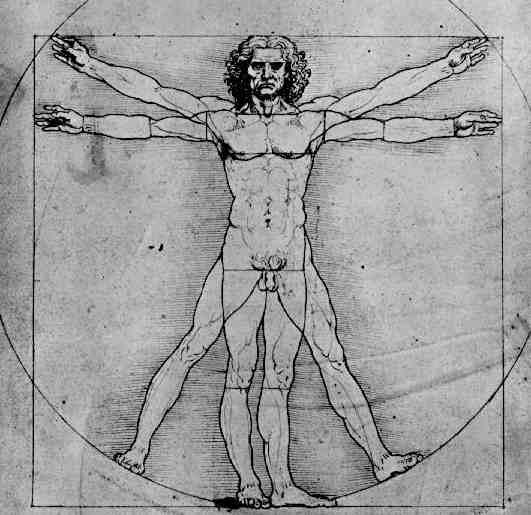
\includegraphics[height=50mm]{Figs/da-vinci-man.jpg}
\end{minipage}
\hspace{15mm}
\begin{minipage}[t]{50mm}
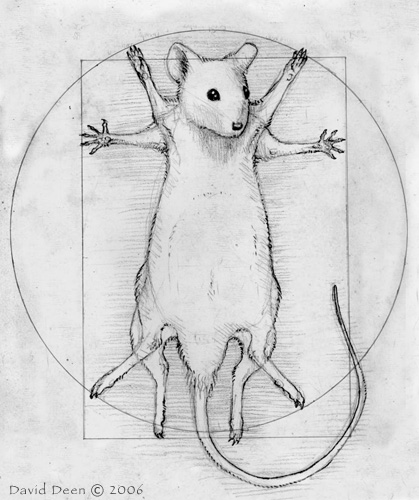
\includegraphics[height=50mm]{Figs/vitruvian_mouse.jpg}
\hspace{5mm}
\href{http://daviddeen.com}{\scriptsize \lolit \tt daviddeen.com}
\end{minipage}
}
\end{frame}


\begin{frame}[c]{Intercross}
\figw{Figs/intercross.pdf}{1.0}
\end{frame}





\begin{frame}[c]{QTL mapping}

\vspace{5mm}
\figw{Figs/lodcurve_insulin_with_effects.pdf}{0.96}
\end{frame}


\begin{frame}[c]{Congenic line/NIL}

\figw{Figs/congenic.pdf}{1.0}

\end{frame}



\begin{frame}[c]{Improving precision}

  \vspace{-20mm}

  \bbi
\item more recombinations
\item more individuals
\item more precise phenotype
\item lower-level phenotypes
\bi
\item transcripts, proteins, metabolites
  \ei
  \ei

\end{frame}



\begin{frame}[c]{Genome-scale phenotypes}

\vspace*{5mm}

\figh{Figs/mouse_on_chips.png}{0.75}
\hfill
\href{https://biochem.wisc.edu/faculty/attie}{\scriptsize \lolit Alan
  Attie} \hspace{8mm}

\end{frame}




\begin{frame}[c]{Advanced intercross lines}

  \figw{Figs/ail.pdf}{1.0}

\end{frame}


\begin{frame}[c]{Recombinant inbred lines}

  \only<1>{\figw{Figs/rilines.pdf}{1.0}}
  \only<2>{\figw{Figs/riself.pdf}{1.0}}

\end{frame}



\begin{frame}[c]{Collaborative Cross}

  \figw{Figs/ri8.pdf}{1.0}

\end{frame}


\begin{frame}[c]{MAGIC}

  \figw{Figs/ri8self.pdf}{1.0}

\end{frame}



\begin{frame}[c]{Heterogeneous stock}

  \vspace{2mm}

  \figh{Figs/hs.pdf}{0.9}

\end{frame}


\begin{frame}[c]{MAGIC is magic}

\vspace{-5mm}

\bbi
\item Genetic diversity

\item High-precision mapping

\item Predictable linkage disequilibrium

\item No rare alleles

\item Phenotype replicates to reduce individual variation

\item Pool phenotypes from multiple labs, environments, treatments

\item Genotype once

\onslide<2->{\item \hilit Cool name}

\ei

\end{frame}






\begin{frame}{MAGIC lines}

 \vspace{5mm}

  \figw{Figs/valdar_genet2006.png}{0.9}

  \vspace{20mm}

\hfill {\footnotesize \href{http://www.genetics.org/content/172/3/1783.full}{\lolit Valdar et al., Genetics 172:1783, 2006}}

\onslide<2->{
  \small {\hilit

  \vspace*{-24mm}
\hspace*{30mm} combine \hspace*{18mm} mix \hspace*{29mm} fix}
}

\onslide<3->{
\vspace*{10pt}
\hspace*{8mm}
How many?
}

\onslide<4->{
\vspace*{8pt}
\hspace*{8mm}
Which?
}

\onslide<5->{
\vspace*{-35pt}
\hspace*{60mm}
How long?
}

\onslide<6->{
\vspace*{-12pt}
\hspace*{100mm}
How?
}

\end{frame}



\begin{frame}[c]{The goal}

Identify QT\only<1>{L}\only<2->{\vhilit G}

\bbi

\item Power
\item Mapping precision
\onslide<3>{\item Estimate QTL allele frequencies}

\ei

\end{frame}




\begin{frame}[c]{Principles}

\bbi

\item Avoid population structure
\item Tradeoff between {\hilit power for \emph{de novo\/} discovery}
  and {\hilit mapping precision}
\item More QTL to find $ \ \Rightarrow \ $ more QTL getting in the way?
\item More QTL alleles $ \ \Rightarrow \ $ less information about each
\item Are QTL alleles common or rare?

\ei

\end{frame}



\begin{frame}{How many founders?}

\vspace{8mm}

  \begin{columns}

    \begin{column}{0.5\textwidth}
      {\hilit More}

{\small
\bi
\item More general use
\item More QTL
\item Greater precision
\item Estimate allele frequencies
\item Haplotype analysis in founders
  \ei
}

    \end{column}

    \begin{column}{0.5\textwidth}
      {\hilit Fewer}

{\small
\bi
\item Lower residual variance
\item Greater power for a particular QTL?
\item Better power for epistasis
\item Rare alleles are less rare
\ei
}
    \end{column}


  \end{columns}


\end{frame}



\begin{frame}[c]{Which founders?}

  \bbi
\item Diverse
\item Interesting
\item No breeding problems
\item Balanced: star phylogeny
  \ei

\end{frame}


\begin{frame}[c]{How much mixing?}

  \bbi
  \item More mixing $ \ \Rightarrow \ $ Greater mapping precision
\item ...but lower power for \emph{de novo\/} mapping
\item Potential for population structure, missing alleles
\item \hilit Random mating or curated mating?
\item \hilit Start with many random cross directions?
  \ei

\end{frame}


\begin{frame}[c]{Selfing or DH?}

\bbi
\item Inbreeding gives added recombination
\item But not so much as at the mixing stage
\item \hilit If doubled haploids are feasible, use them
  \ei

\end{frame}




\begin{frame}[c]{Sharing is also key}

\bbi
\item The greatest power of MAGIC comes from sharing
  \bi
\item[] \hilit Pooling data, exploring multiple environments/treatments
  \ei

\item Common software needs
  \bi
\item[] \hilit Analysis software, database infrastructure
  \ei

\item Many students need to learn the same stuff
  \bi
\item[] \hilit Joint training opportunities
  \ei

  \ei

\end{frame}





\begin{frame}{Summary}

  \bbi
\item How many founders?
  \bi
\item Tradeoff between {\hilit diversity} and information about
  {\hilit particular alleles}
  \ei

\item Which founders?
  \bi
\item Diverse, interesting, no breeding problems, star phylogeny
  \ei

\item How long to mix?
  \bi
\item Tradeoff between {\hilit power} and {\hilit precision}
  \ei


\item How to fix?
  \bi
\item Doubled haploids are great if feasible
  \ei


\item Let's share!
  \bi
\item Lines, data, software, training
  \ei



  \ei


\end{frame}



\begin{frame}[c]{}

\Large

Slides: \href{https://kbroman.org/Talk_MAGIC2021}{\tt
  kbroman.org/Talk\_MAGIC2021} \quad
\includegraphics[height=5mm]{Figs/cc-zero.png}

\vspace{7mm}

\href{https://kbroman.org}{\tt \lolit kbroman.org}

\vspace{7mm}

\href{https://kbroman.org/qtl2}{\tt kbroman.org/qtl2}

\vspace{7mm}

\href{https://github.com/kbroman}{\tt \lolit github.com/kbroman}

\vspace{7mm}

\href{https://twitter.com/kwbroman}{\tt \lolit @kwbroman}


\end{frame}

\end{document}
